\chapter{Introduction}
\label{chap:intro}
\section{Background}
\label{sec:background}
The automotive market share held by hybrid and electric vehicles is growing.
This growth is mainly possible thanks to advances in energy storage technologies and manufacturing processes.
While there are many environmental advantages, an electric powertrain also offers greater flexibility during the design process of the automobile.

In comparison to similarly performing internal combustion engines, electric motors are smaller and simpler as they have only one moving part that is the rotor and driveshaft assembly, this makes it possible to use more than one motor without adding too much manufacturing complexity.

Using one motor for each driven wheel can reduce the size, weight and complexity of the trasmission. This is beacuse mechanical power can be produced closer to the wheels and the need for differentials is eliminated.

These motors may also be individually controlled to produce different amounts of torque (see figure \ref{rimac}) resulting in moment about the vertical (yaw) axis, this kind of control strategy is called torque vectoring. Torque vectoring may be used to correct an oversteering or understeering vehicle, benefitting consumer vehicles with increased safety and race cars with improved handling.

Individual wheel traction control is also possible, allowing greater cornering speed in the racing environments that allow it.

\begin{figure}[tb]
  \centering
  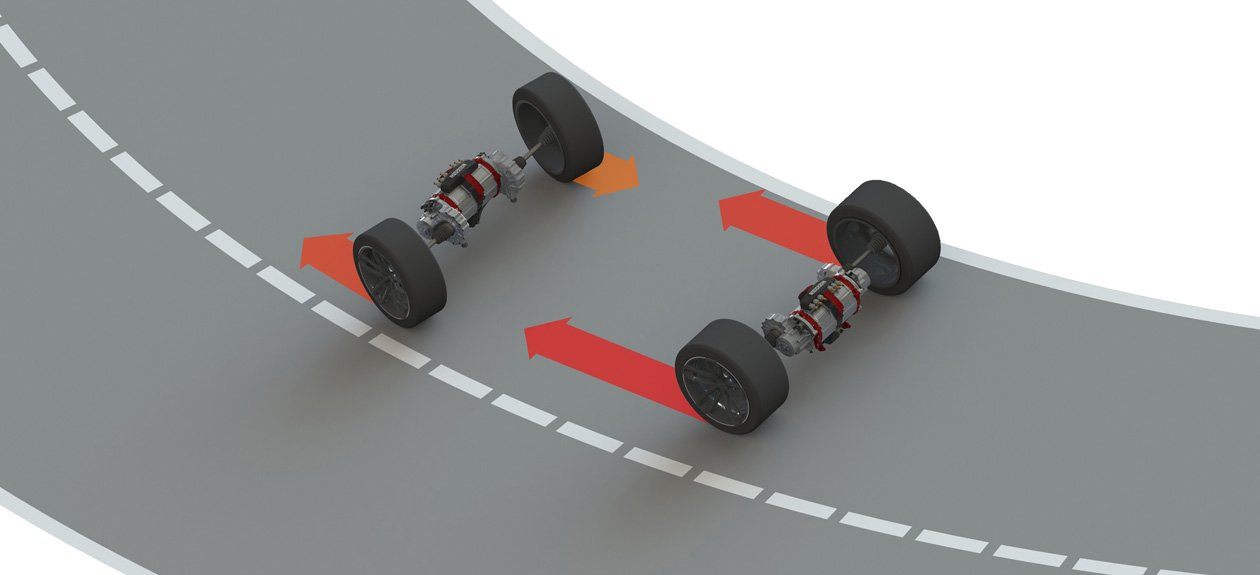
\includegraphics[width=\textwidth]{images/rimac.jpg}
  \caption{The Rimac Concept One EV powertrain applying different amounts of force at each road contact point.}
  \label{rimac}
\end{figure}

\section{Objectives}
\label{sec:objectives}
The objective of the present work is to derive a mathematical model to be used  in simulations and in the development of control algorithms for traction control and torque vectoring applications in electric vehicles.
Future participation in the Formula Student electric competitions has been the main motivation behind the development of the model. It is therefore conceived with racing in mind. The tipically high suspension stiffness of cars competing in this category is taken into account when making approximations.

Modelling of the roll dynamics renders lateral load transfer transients predictable, allowing for greater accuracy in high frequency manouvers such as lane changes, small chicanes and slaloms which make up the Formula Student Autocross and Endurance courses (like the one shown in figure \ref{autox}).


\begin{figure}[tb]
  \centering
  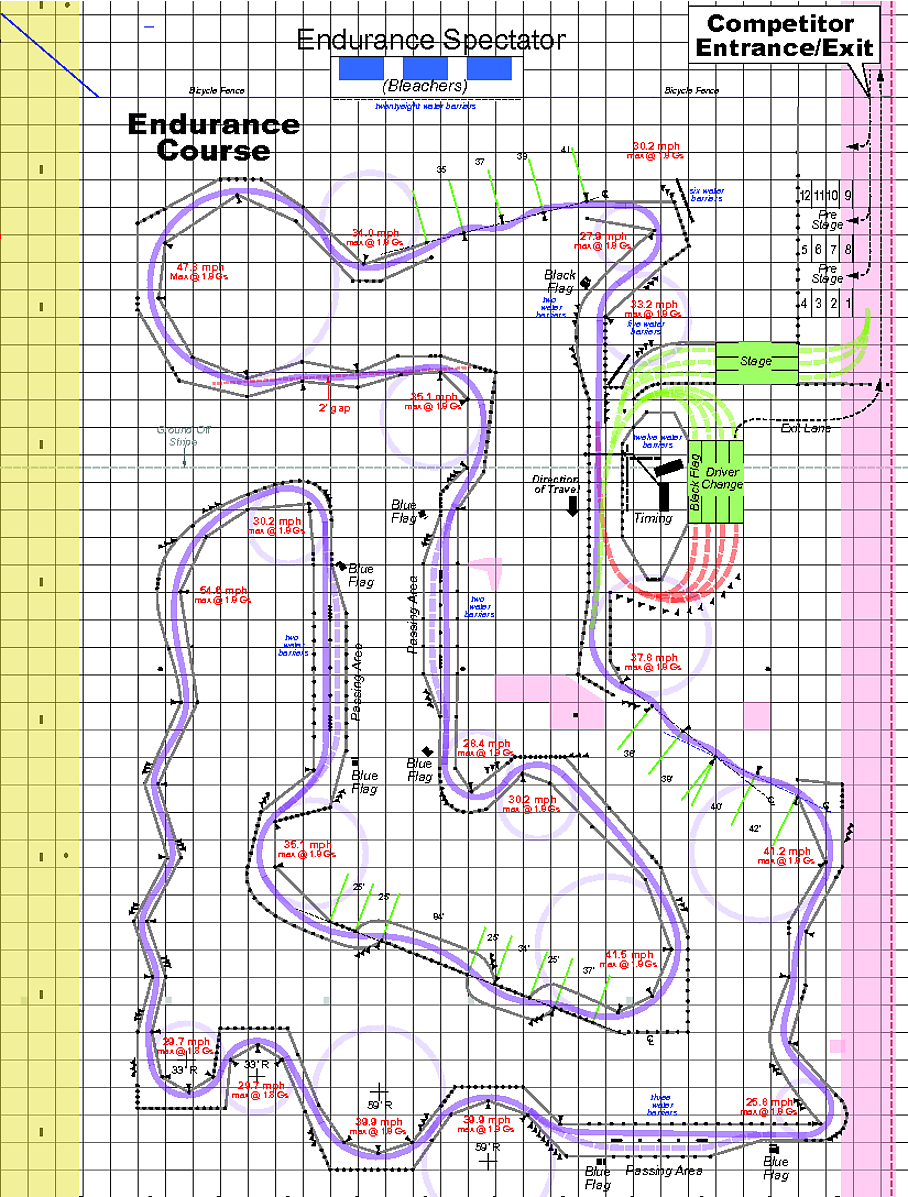
\includegraphics[height=15cm]{images/autox}
  \caption{Example of a Formula SAE Endurance Course.}
  \label{autox}
\end{figure}

Inclusion of the roll and pitch behaviour in the models also allows correlation of vertical forces to the suspension travel, the latter being an easily measurable physical quantity that can be added as an input to the vehicle control system.

The rear steering dynamics were included in the second model as Formula Student rules explicitly allow it and their modelling did not cost any extra effort.

\section{Approach}
\label{sec:approach}
In Chapter \ref{chap:6dof} a 6 degree-of-freedom model is physically and mathematically described. The lagrange formulation of the system is then given. Chapter \ref{chap:12dof} extends the model reaching 12 degrees-of-freedom to describe the four wheel rotations and the front and rear steering dynamics.
The Lagrange formulation is symbolically constructed using the MATLAB Symbolic Math Toolbox to facilitate co-ordinate transformations and differentiations.
Functions were written to algebraically solve the Lagrange Equations and generate the state space representation of the system.
All scripts are written in vectorial form allowing for compact and more readable code.
Simulations were run in the Simulink environment with a 2D graphical representation of the car as a troubleshooting tool.
A brief overview of tyre modelling was required in order to run realistic simulations.
